\paragraph{Sơ đồ tuần tự luồng khởi tạo giao dịch mua gói thuê bao VIP}

Luồng nghiệp vụ này mô tả
bước người dùng
chọn gói thuê bao VIP trên Web Frontend,
hệ thống kiểm tra gói dịch vụ,
chuẩn bị Subscription, tạo Transaction ở trạng thái \texttt{pending},
đăng ký job timeout trên Redis BullMQ,
sau đó gọi cổng thanh toán để sinh đường link thanh toán.

\begin{figure}[H]
\centering
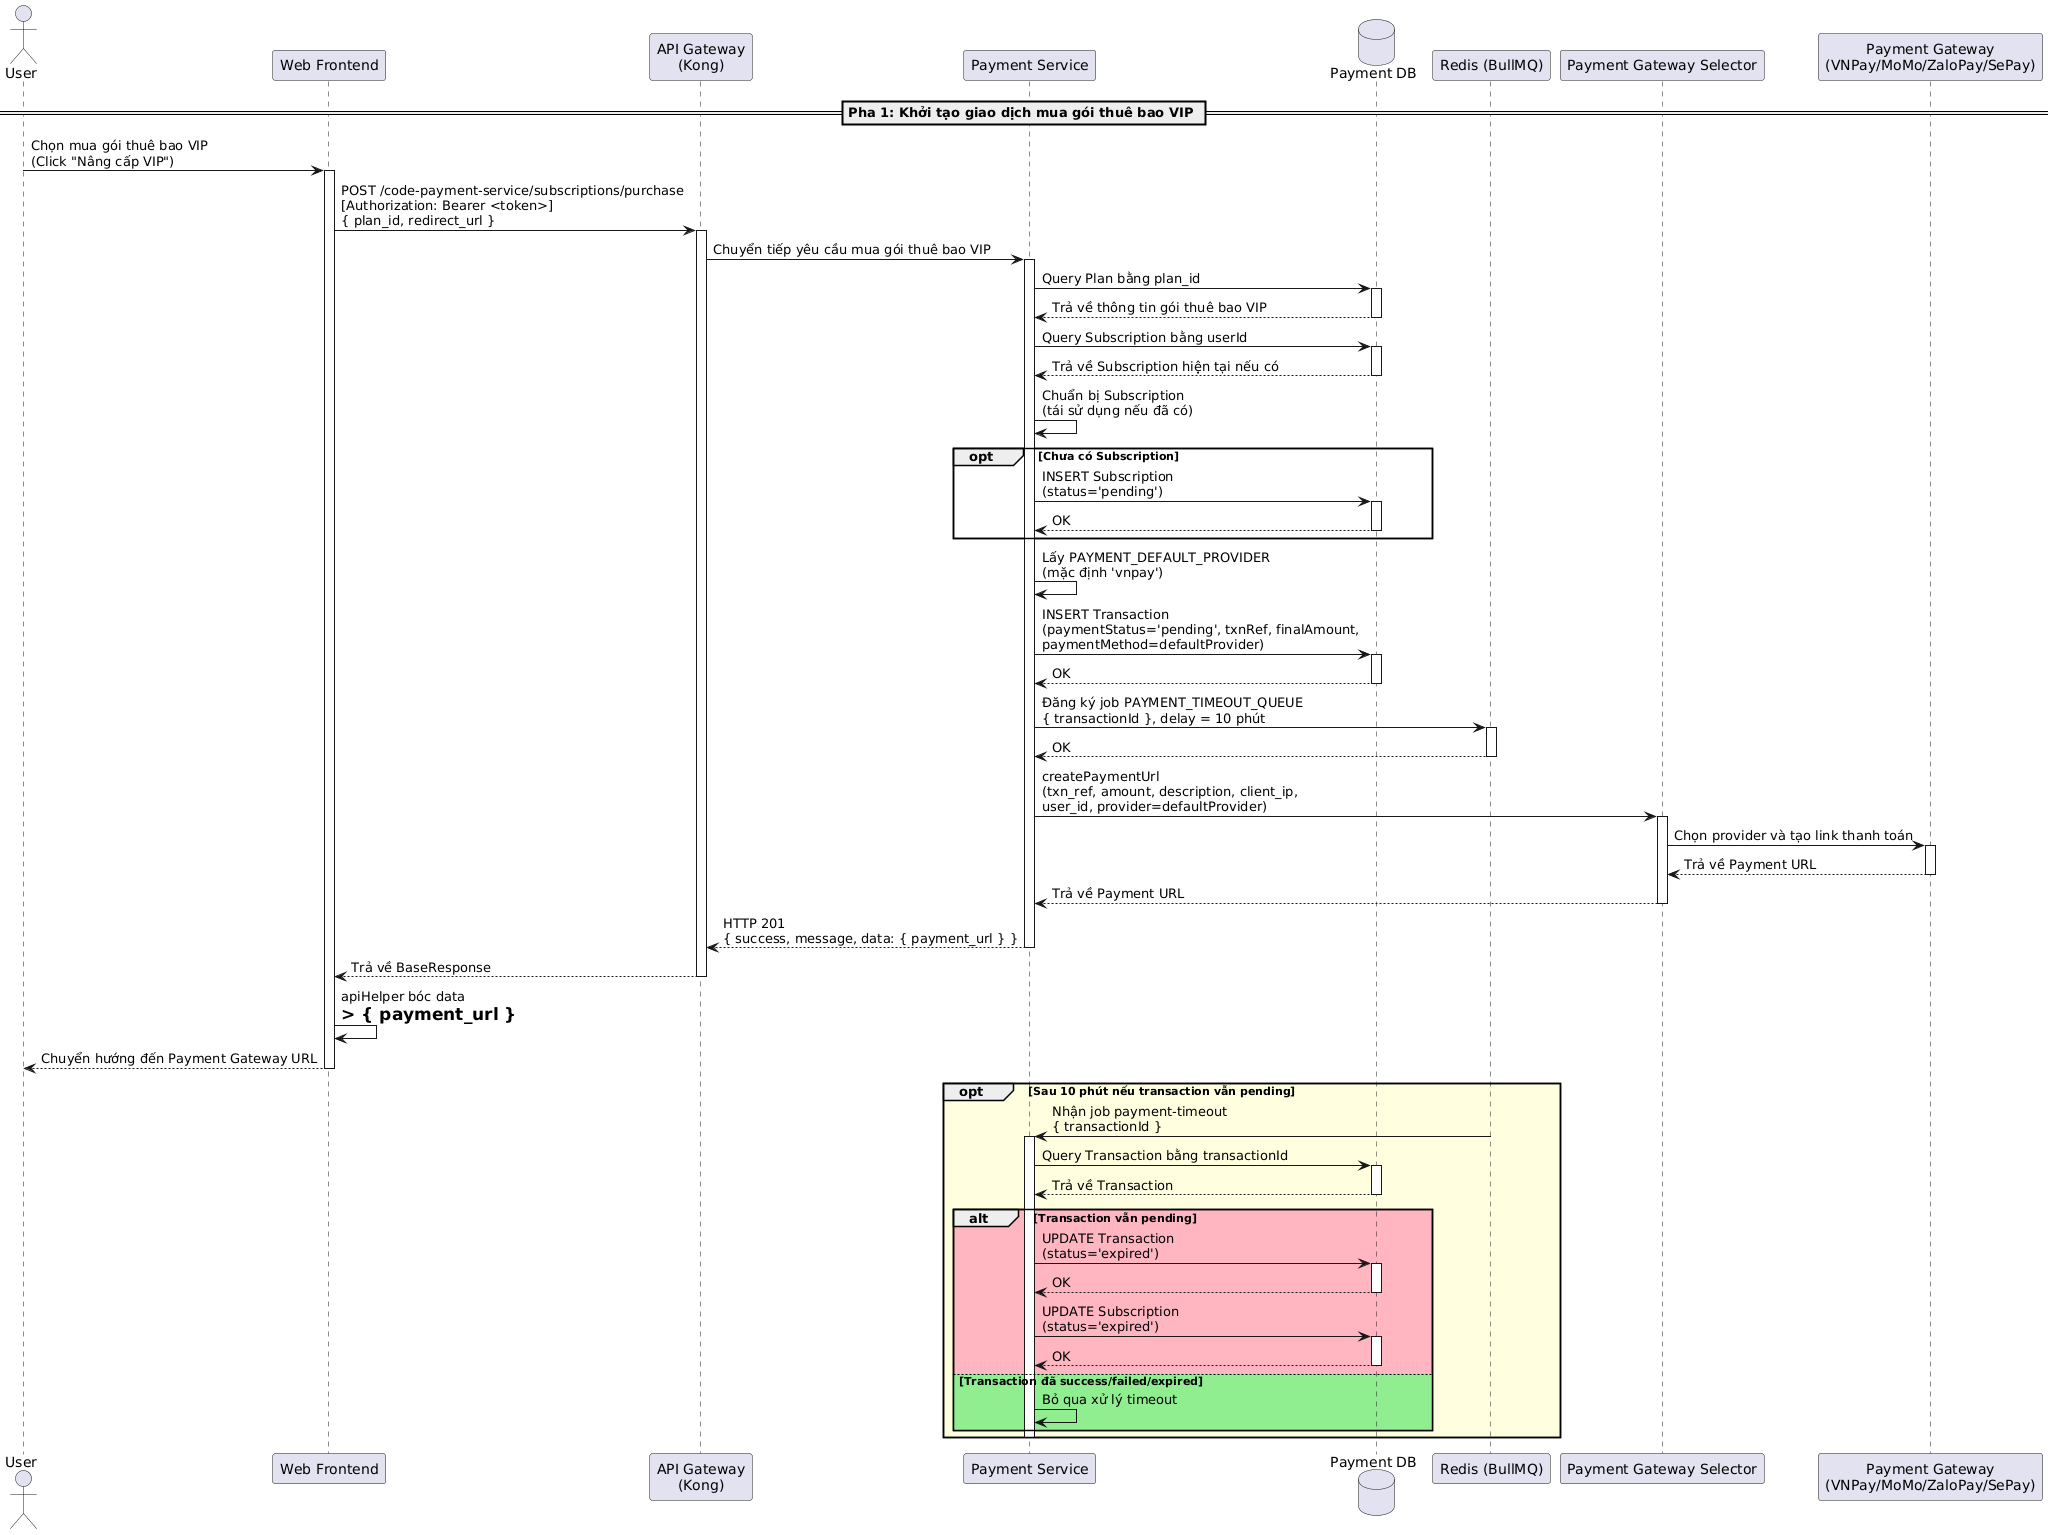
\includegraphics[width=0.95\textwidth]{contents/Sequence/UML-Sequence-UserCreateVipPaymentTransaction.png}
\caption{Sơ đồ tuần tự luồng khởi tạo giao dịch mua gói thuê bao VIP}
\end{figure}

\begin{table}[H]
\centering
\renewcommand{\arraystretch}{1.3}

\begin{tabular}{|l|l|p{5cm}|}
\hline
\textbf{Thành phần} & \textbf{Phân loại} & \textbf{Vai trò trong hệ thống} \\ \hline
User & Actor & Người dùng đã đăng nhập và chọn mua gói thuê bao VIP. \\ \hline
Web Frontend & Component & Giao diện web Next.js. \\ \hline
API Gateway (Kong) & Component & Cổng API chuyển tiếp các yêu cầu API. \\ \hline
Payment Service & Microservice & Kiểm tra plan, chuẩn bị subscription, tạo transaction, đăng ký timeout job và yêu cầu link thanh toán từ gateway provider mặc định. \\ \hline
Payment DB & Database & Lưu thông tin gói thuê bao VIP, subscription và transaction. \\ \hline
Redis (BullMQ) & Component & Quản lý job để hết hạn giao dịch sau 10 phút. \\ \hline
Payment Selector & Component & Chọn cổng thanh toán, mặc định là \texttt{vnpay}. \\ \hline
Payment Gateway & External Service & Cổng thanh toán bên thứ ba sinh Payment URL, hiện có các adapter VNPay, MoMo, ZaloPay và SePay. \\ \hline
\end{tabular}
\caption{Các thành phần tham gia luồng khởi tạo giao dịch mua gói thuê bao VIP}
\end{table}

\subparagraph{Mô tả tổng quan}

\begin{itemize}

\item \textbf{Yêu cầu nâng cấp:}
Người dùng chọn nâng cấp gói thuê bao VIP trên giao diện,
giao diện gửi yêu cầu đăng ký mua gói thuê bao VIP
qua cổng API với thông tin định danh gói dịch vụ
và địa chỉ chuyển hướng sau khi thanh toán.

\item \textbf{Kiểm tra gói dịch vụ:}
Dịch vụ thanh toán
kiểm tra gói dịch vụ còn đang hoạt động hay không,
tìm kiếm gói thuê bao VIP hiện tại của người dùng
để cập nhật hoặc tạo mới gói thuê bao VIP
ở trạng thái chờ thanh toán nếu chưa có.

\item \textbf{Khởi tạo giao dịch thanh toán:}
Dịch vụ thiết lập cổng thanh toán mặc định,
tạo một giao dịch thanh toán mới trong CSDL
và đăng ký một công việc kiểm tra hết hạn giao dịch sau 10 phút
vào hàng đợi Redis.

\item \textbf{Tạo liên kết thanh toán:}
Dịch vụ kết nối
với cổng thanh toán để tạo liên kết thanh toán.
Giao diện tiếp nhận thông tin
và nhận trực tiếp liên kết thanh toán
để điều hướng người dùng.

\item \textbf{Xử lý hết hạn:}
Bộ xử lý công việc hết hạn sẽ kiểm tra sau 10 phút:
nếu giao dịch vẫn ở trạng thái chờ thanh toán
thì cập nhật giao dịch và gói thuê bao VIP liên quan thành hết hạn.
Nếu giao dịch đã ở các trạng thái thành công, thất bại hoặc đã hết hạn trước đó thì bỏ qua công việc này.
\end{itemize}
